%! Author = jbf
%! Date = 31.07.25

\newpage
\section{Grundlagen}
\label{Grundlagen}

\subsection{Überblick über den Umrichter-Prüfstand}
In diesem Unterkapitel wird der Umrichter-Teststand, von dem die zu verarbeitenden Datensätze stammen beschrieben,
da dies für das generelle Verständnis der einzulernenden Datensatzstruktur unerlässlich ist.
Die genaue Bezeichnung des Teststandes „USTB DWT Test Bench (XCT0006-1)“ im weiteren als Test-Bench oder Teststand benannt.
Diese Art Teststand wird im allgemein für die End-of-Line Prüfung von unterschiedlichen Umrichtern nach ihrer Herstellung genutzt,
um die Produktqualität und -funktionalität sicherzustellen.

In dem hier vorliegenden Fall wird der Teststand verwendet, um die aus dem Feld kommenden Umrichter auf ihre weiter Nutzungstauglichkeit zu testen.
Die weiter Nutzungstauglichkeit wird ermittelt, indem die Messwerte mit Mittelwerten, die von mehreren fabrikneuen Umrichtern stammenden verglichen werden.
Diese Messwerte müssen sich in einen vorher definierten Toleranzbereich befinden um weiter verwenden zu werden.

Die Test-Bench besteht aus mehreren Hauptkomponenten:

\begin{itemize}
\item Das Netzteil, welches mit einer 400V Netzspannung versorgt wird, wandelt diese in eine Gleichspannung. Das Netzteil leifert maximal 8kW mit 1200VDC oder 800VDC, welche Werte verwendet werden kann vor Teststart bestimmt werden. In Abbildung 1\ref{fig:1. Aufbau des Teststandes} mit PSU bezeichnet, für „Power Supply Unit“.


\item Das Elektronik-Rack, auf dem Mess- und Control-Komponenten befestigt sind. Hier befinden sich auch der (XCS2100) System-Controller der das ganze System mit dem PC, auf dem die Test-Bench Software läuft, via Ethernet verbindet. In Abbildung \ref{fig:1. Aufbau des Teststandes} mit ER bezeichnet, für „Electronic Rack“.


\item Der Testmatrix-Schrank, in dem die Sammelschienen für den Stromanschluss und den Schützen sitzen. In Abbildung \ref{fig:1. Aufbau des Teststandes} mit TM bezeichnet, für „Test Matrix cabine“.


\item Der Schrank mit dem Kühlungssystem, da die Umrichter während des Betriebes Wassergekühlt werden müssen. In Abbildung \ref{fig:1. Aufbau des Teststandes} mit „Cool1“ bezeichnet.


\item Dem Carrier, auf dem Umrichter befestigt werden. Dieser wird speziell für bestimmte Umrichter konstruiert. In Abbildung \ref{fig:1. Aufbau des Teststandes} mit Carrier1 bezeichnet.

\end{itemize}

\begin{figure}[h]
    \centering
    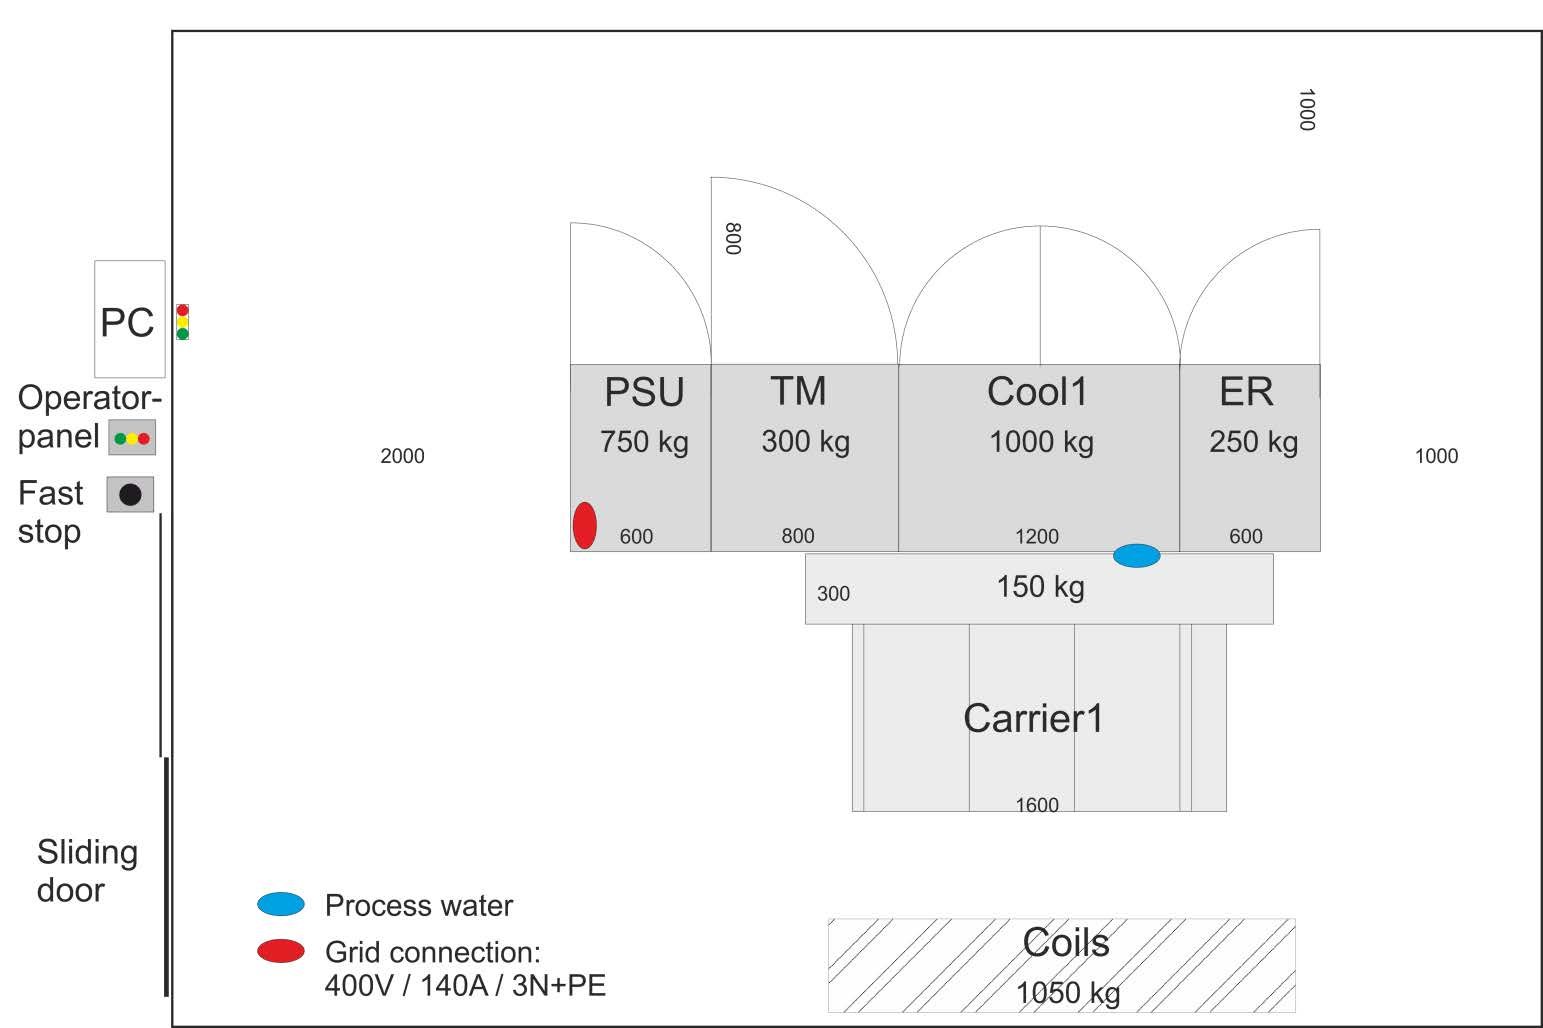
\includegraphics[width=0.8\textwidth]{Grafiken/Test Cabin.jpg}
    \caption{Aufbau des Teststandes- kopiert aus KkKKK}
    \label{fig:1. Aufbau des Teststandes}
\end{figure}

Neben dem Hauptkomponenten befinden sich außerhalb des Sicherheitsbereiches, der während des Betriebes nicht betreten werden darf,
ein PC mit einer Software zum Steuern der Testeinrichtung, sowie eine Betriebsanzeige und ein Notaus.

\newpage

Ein Test läuft wie folgt ab:

\begin{enumerate}
\item Die Umrichter werden auf dem Carrier befestigt, es werden meist 3 Umrichter gleichzeitig getastet, Abweichungen je nach Bauform der Umrichter.
Ab diesem Zeitpunkt werden die Umrichter in der gegebenen Fachliteratur als DUTs „Devices-Under-Test“ bezeichnet, dies kommt auch in den Testberichten vor,daher hat der Autor diesen Begriff einzuführen und fortan zu übernehmen.


\item Durchführung des Driver Consumption Testes.


\item Durchführung des Pulse Testes.


\item Durchführung des Driver Power Testes.


\item Nach dem Durchlaufen eines Tests wird automatische ein XML-Datenfile mit den erhobenen Messdaten generiert, die enthalt die Messwerte und alle vorher bestimmten Einstellungen.


\end{enumerate}
Es gibt verschiedene Testmodule, die auf dem Teststand laufen. Einige der verschiedenen Funktionen eines DUT können mit dem gleichen Modus eines Testmoduls überprüft werden, indem die entsprechenden Parametersätze ausgewählt werden. Jeder Test ist autonom und kann mehrmals ausgeführt werden, auch mit unterschiedlichen Parametersätzen. Im Folgenden wird eine kurze Beschreibung der Funktionen der für diese Arbeit relevanten Testmoduls gegeben.

DRIVER CONSUMPTION TEST

The driver current consumption test verifies the driver´s current consumption in idle state and during PWM-Switching.

PULSE TEST

The pulse test has three function modes:

- In mode Functional-Switching (FSW) it can be checked, if the semiconductors are switching in general. \\
- In mode Over-Current-Protection (OCP) the over-current monitoring (“soft short circuit”) can be checked.\\
- In mode Dynamic-Short-Circuit-Protection (DSCP) the correct behavior of the driver stage is checked in respect of a hard short circuit.

POWER TEST

With this test, two different features can be tested:

- On the one hand the Burn-In-Test (BIT) is suited for operating the DUTs in a cyclic manner and hence simulating real operational states.
On the other hand by checking the cooling temperature at the end of test the correct heat transfer of the semiconductors can be verified.\\
During Over-Temperature-Protection test (OTP) a DUT is run on reduced cooling until the maximum permissible heat sink temperature is reached and the temperature protection circuit trips.


\subsection{Verarbeitung von XML-Daten}

\subsection{Datenbankentwurf und Normalisierung}

\subsection{Grundlagen der Datenvisualisierung}

\subsection{Anforderungen an modulare Softwareentwicklung}